%************************************************
\chapter{Tensorflow basics}\label{ch:tensorflow_basics}

\ac{TF} is an open source software library for machine learning in various kinds of perceptual and language understanding tasks. It is currently used for both research and production by different teams in dozens of commercial Google products [\cite{DBLP:journals/corr/AbadiABBCCCDDDG16}], such as speech recognition, Gmail, Google Photos, and Google Search, many of which had previously used its predecessor DistBelief [\cite{40565}]. 

\href{https://www.tensorflow.org/}{TensorFlow} was originally developed by the Google Brain team for Google's research and production purposes and later released under the Apache 2.0 open source license on November 9, 2015.  Many teams nowadays at Google have migrated from DistBelief to TensorFlow for research and production uses.

This library of algorithms originated from Google's need to instruct neural networks, to learn and reason similarly to how humans do, so that new applications can be derived which are able to assume roles and functions previously reserved only for capable humans; the name TensorFlow itself derives from the operations which such neural networks perform on multidimensional data arrays. These multidimensional arrays are referred to as "tensors" but this concept is not identical to the mathematical concept of tensors. Its purpose is to train neural networks to detect and decipher patterns and correlations.

The aim of this chapter is to present the main data structures and operations provided by \acs{TF} as well as to explain their basic usage. In particular the notions of computation graph, constant, variable and feed will be explained. Then, TensorBoard, a powerful tool for visualizing learning, will be presented. Finally, the last section includes a very simple example model built using TensorFlow.

The material provided in this chapter is taken form [\cite{tensorflow}].

\section{Overview}

TensorFlow is Google Brain's second generation machine learning system. While the reference implementation runs on single devices, \ac{TF} can run on multiple \acsp{CPU} and \acsp{GPU} (with optional \acs{CUDA} extensions for general-purpose computing on graphics processing units). It runs on 64-bit Linux or Mac OS X desktop or server systems, as well as on mobile computing platforms, including Android and Apple's iOS.

It provides a Python API, as well as a less documented C++ API. In particular, the TensorFlow Python API supports Python 2.7 and Python 3.3+. It can be easily installed as a common Python package through \lstinline|pip| or in Anaconda with a \lstinline|conda| installation.

TensorFlow computations are expressed as stateful dataflow \textbf{graphs}. Nodes in the graph are called \emph{ops} (\ie operations). An op takes zero or more \lstinline|Tensor| objects, performs some computation, and produces zero or more \lstinline|Tensors|. In TensorFlow terminology, a Tensor is simply a typed multi-dimensional array. For instance, a batch of images can be represented as a 4D tensor \lstinline|Tensor| of floating point numbers with dimensions \lstinline|[batch, height, width, channels]|.

In other words, a \ac{TF} graph is a description of some computations. In order to actually compute anything, a graph must be launched in a \lstinline|Session|. A \lstinline|Session| object places the graph ops onto \lstinline|Devices|, \ie \acsp{CPU} or \acsp{GPU} and provides methods to execute them. In Python, these methods return tensors produced by ops as numpy \lstinline|ndarray| objects.

\section{The computation graph}

TensorFlow programs are usually structured into a construction phase, that assembles a graph, and an execution phase that uses a session to execute ops in the graph.

For example, it is common to create a graph to represent a neural network in the construction phase, and then repeatedly execute a set of training ops in the graph in the execution phase.

\subsection{Building the graph}

To build a graph it's useful start with ops that do not need any input (source ops), such as \lstinline|Constant|, and pass their output to other ops that do computation. The ops constructors in the Python library return objects that stand for the output of the constructed ops. You can pass these to other ops constructors to use as inputs.

The TensorFlow Python library has a default graph to which ops constructors add nodes that is sufficient for many applications. However, it is possible to explicitly manage multiple graphs.

The following code builds a graph composed by three nodes. The two \lstinline|constant()| operations produce two matrices (a $1x2$ and a $2x1$ matrix), while the \lstinline|matmul()| operation takes as input the two previously created matrices and outputs the result of the matrix multiplication.

\begin{lstlisting}
import tensorflow as tf

matrix1 = tf.constant([[3., 3.]])
matrix2 = tf.constant([[2.],[2.]])

product = tf.matmul(matrix1, matrix2)
\end{lstlisting}

In order to actually multiply the matrices, and get the result of the multiplication, the graph must be launched in a \lstinline|Session|.

\subsection{Launching the graph}

Launching follows construction. To launch a graph, a \lstinline|Session| object. Without arguments the session constructor launches the default graph.

The following code creates a session, launches the previously created graph and prints he result of the matrix multiplication.

\begin{lstlisting}
# Launch the default graph
sess = tf.Session()

result = sess.run(product)
print(result)
# ==> [[ 12.]]

# Close the Session when we're done
sess.close()
\end{lstlisting}

To run the matmul op we call the session \lstinline|run()| method, passing \lstinline|product| which represents the output of the \lstinline|matmul| op. This indicates to the call that we want to get the output of the \lstinline|matmul| op back. All inputs needed by the op are run automatically by the session, typically in parallel. The call \lstinline|run(product)| thus causes the execution of three ops in the graph: the two \lstinline|constants| and \lstinline|matmul|. The output of the matrix multiplication is returned in \lstinline|result|.

Sessions should always be closed to release resources.  They can be also surrounded with a \lstinline|with| block. In this way, the \lstinline|Session| closes automatically at the end of the block. The code then becomes:

\begin{lstlisting}
with tf.Session() as sess:
    result = sess.run([product])
    print(result)
\end{lstlisting}

\section{Variables}

\lstinline|Variable| objects maintain state across executions of the graph. When a model is trained, \lstinline|Variables| are used to hold and update parameters. They are in-memory buffers containing tensors. They must be explicitly initialized and can be saved to disk during and after training. Saved values can be later restored to exercise or analyze the model.

\subsection{Creation}

When a \lstinline|Variable| a \lstinline|Tensor| is passed to the \lstinline|Variable()| constructor as initial value. \acs{TF} provides a collection of ops that produce tensors that can be used for initialization from constants or random values. All these ops require to specify the shape of the tensors. That shape automatically becomes the shape of the variable. Variables generally have a fixed shape, but TensorFlow provides advanced mechanisms to reshape them.

The following code creates two variables, one for weights and one for biases.

\begin{lstlisting}
weights = tf.Variable(tf.random_normal([784, 200], stddev=0.35),
                      name="weights")
biases = tf.Variable(tf.zeros([200]), name="biases")
\end{lstlisting}

Calling \lstinline|tf.Variable()| adds several ops to the graph:

\begin{itemize}
	\item A \lstinline|Variable| op the holds the variable value;
	\item An initializer op that sets the variable to its initial value;
	\item The ops for the initial value (\eg the \lstinline|zeros| op for \lstinline|biases|).
\end{itemize}

The output is an instance of the Python class \lstinline|tf.Variable|.

\subsection{Initialization}

Variable initializers must be run explicitly before other ops in the model can be run. The easiest way to do that is to add an op that runs all the variable initializers, and run that op before using the model.

The op \lstinline|tf.global_variables_initializer()| can be used to add an op to run variable initializers. The op must be run after the model has been fully constructed.

The following code initializes the two variables created before:

\begin{lstlisting}
init_op = tf.global_variables_initializer()

with tf.Session() as sess:
    # Run the init operation.
    sess.run(init_op)
    ...
\end{lstlisting}

\subsection{Saving and restoring}

The easiest way to save and restore a model is to use a \lstinline|tf.train.Saver| object. The constructor adds \lstinline|save| and \lstinline|restore| ops to the graph for all, or a specified list, of the variables in the graph. The saver object provides methods to run these ops, specifying paths for the checkpoint files to write to or read from.

Checkpoints are binary files that, roughly, contain a map from variable names to tensor values.

The same \lstinline|tf.train.Saver()| object can be used to manage all the variables in the model. Restored variables do not have to be initialized beforehand.

The following two pieces of code save and restore two variables:

\begin{lstlisting}
v1 = tf.Variable(..., name="v1")
v2 = tf.Variable(..., name="v2")

init_op = tf.global_variables_initializer()

saver = tf.train.Saver()

with tf.Session() as sess:
    sess.run(init_op)
    ...
    save_path = saver.save(sess, "/tmp/model.ckpt")
    print("Model saved in file: %s" % save_path)
\end{lstlisting}

\begin{lstlisting}
v1 = tf.Variable(..., name="v1")
v2 = tf.Variable(..., name="v2")

saver = tf.train.Saver()

with tf.Session() as sess:
    saver.restore(sess, "/tmp/model.ckpt")
    print("Model restored.")
    ...
\end{lstlisting}

If no argument is passed to \lstinline|tf.train.Saver()|, the saver handles all variables in the graph. Each one of them is saved under the name that was passed when the variable was created.

It is sometimes useful to explicitly specify names for variables in the checkpoint files. For example, there might be a trained model with a variable named "weights" whose value have to be to restored in a new variable named "params".

It is also sometimes useful to only save or restore a subset of the variables used by a model. For example, a neural net with 5 layers could have been trained. In order to train a new model with 6 layers, the parameters from the 5 layers of the previously trained model can be restored into the first 5 layers of the new model.

The names and variables to save can be easily specified by passing to the \lstinline|tf.train.Saver()| constructor a Python dictionary: keys are the names to use, values are the variables to manage.

\section{Feeds}

The examples above introduced tensors into the computation graph by storing them in constants and variables. \acs{TF} also provides a feed mechanism for patching a tensor directly into any operation in the graph.

A feed temporarily replaces the output of an operation with a tensor value. Deed data are supplied as an argument to a \lstinline|run()| call. The feed is only used for the run call to which it is passed.

The most common use case involves designating specific operations to be "feed" operations by using \lstinline|tf.placeholder()| to create them:

\begin{lstlisting}
input1 = tf.placeholder(tf.float32)
input2 = tf.placeholder(tf.float32)
output = tf.mul(input1, input2)

with tf.Session() as sess:
    sess.run([output], feed_dict={input1:[7.], input2:[2.]})
\end{lstlisting}

A \lstinline|placeholder()| operation generates an error if a feed for it isn't supplied.

\section{Tensorboard}

The computations performed with TensorFlow - like training a massive deep neural network - can be complex and confusing. To make them easier to understand, debug, and optimize TensorFlow programs, the developers included a suite of visualization tools called TensorBoard. It can be used to visualize a TensorFlow graph, plot quantitative metrics about the execution, and show additional data like images that pass through the graph.

TensorBoard operates by reading TensorFlow events files, which contain summary data that can be generated when running a TensorFlow graph.

\begin{figure}
	\centering
	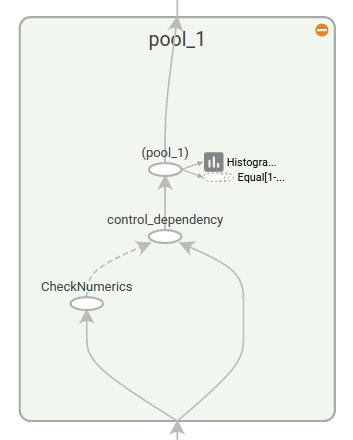
\includegraphics[width=0.5\textwidth]{Images/tensorboard}
	\caption{Graph visualization using TensorBoard}\label{fig:tensorboard}
\end{figure}

Figure \ref{fig:tensorboard} shows an example of graph visualization using this tool. Every node can be expanded or minimized in order to analyze the graph at different granularities.

Further information about the usage of TensorBoard are are available in the \href{https://www.tensorflow.org/how_tos/summaries_and_tensorboard/}{dedicated page on the TensorFlow website}.

\section{A very simple model}

We conclude this chapter showing a very simple linear model built with \acs{TF}.  The program makes up some data in two dimensions, and then fits a line to them.

\begin{lstlisting}
import tensorflow as tf
import numpy as np

# Create 100 phony x, y data points in NumPy, y = x * 0.1 + 0.3
x_data = np.random.rand(100).astype(np.float32)
y_data = x_data * 0.1 + 0.3

# Try to find values for W and b so that y_data = W * x_data + b
# (We know that W should be 0.1 and b 0.3, but TensorFlow will
# figure that out for us.)
W = tf.Variable(tf.random_uniform([1], -1.0, 1.0))
b = tf.Variable(tf.zeros([1]))
y = W * x_data + b

# Minimize the mean squared errors.
loss = tf.reduce_mean(tf.square(y - y_data))
optimizer = tf.train.GradientDescentOptimizer(0.5)
train = optimizer.minimize(loss)

# Before starting, initialize the variables.
init = tf.global_variables_initializer()

# Launch the graph.
sess = tf.Session()
sess.run(init)

# Fit the line.
for step in range(201):
    sess.run(train)
    if step % 20 == 0:
    print(step, sess.run(W), sess.run(b))

# Learns best fit is W: [0.1], b: [0.3]
\end{lstlisting}

The first part of the code builds the data flow graph. TensorFlow does not actually run any computation until the session is created and the run function is called, in the second part of the code.